% Native editable composition from verified, unchanged IDE images.
\par
\begin{figure}[htbp]
\centering
\sbox0{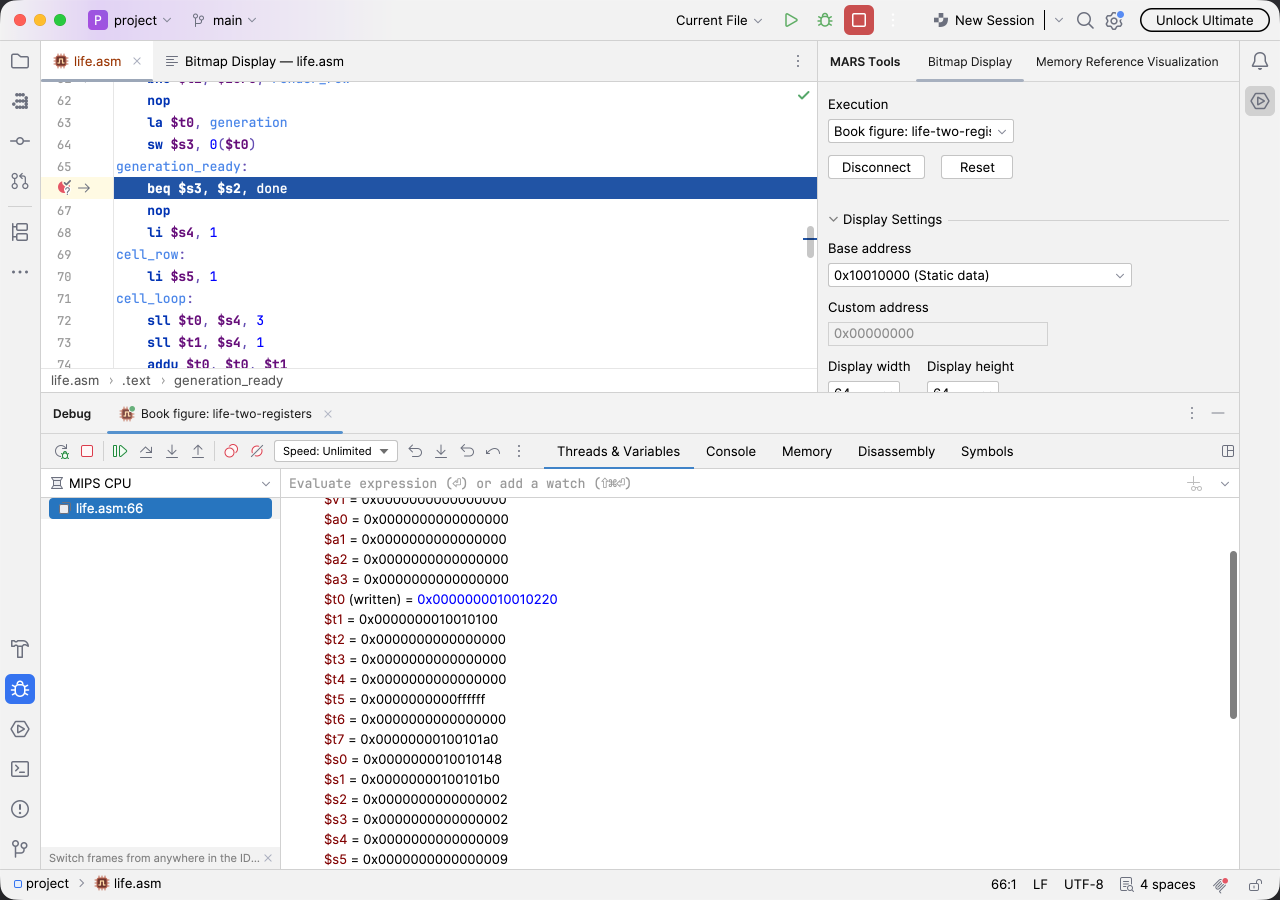
\includegraphics[artifact]{packages/008-life-generations/captures/f04-two/registers.png}}
\sbox2{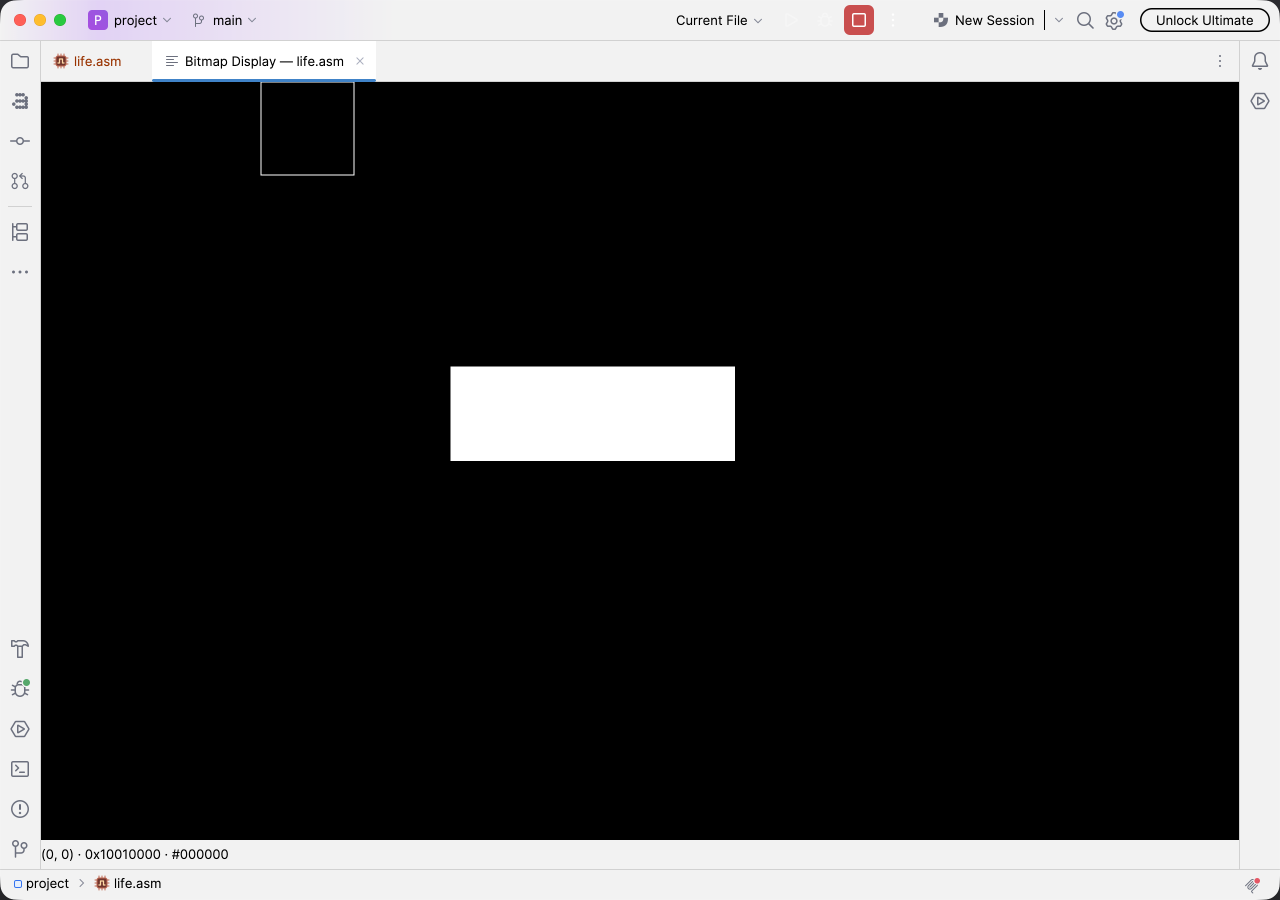
\includegraphics[artifact]{packages/008-life-generations/captures/f04-two/bitmap.png}}
\sbox4{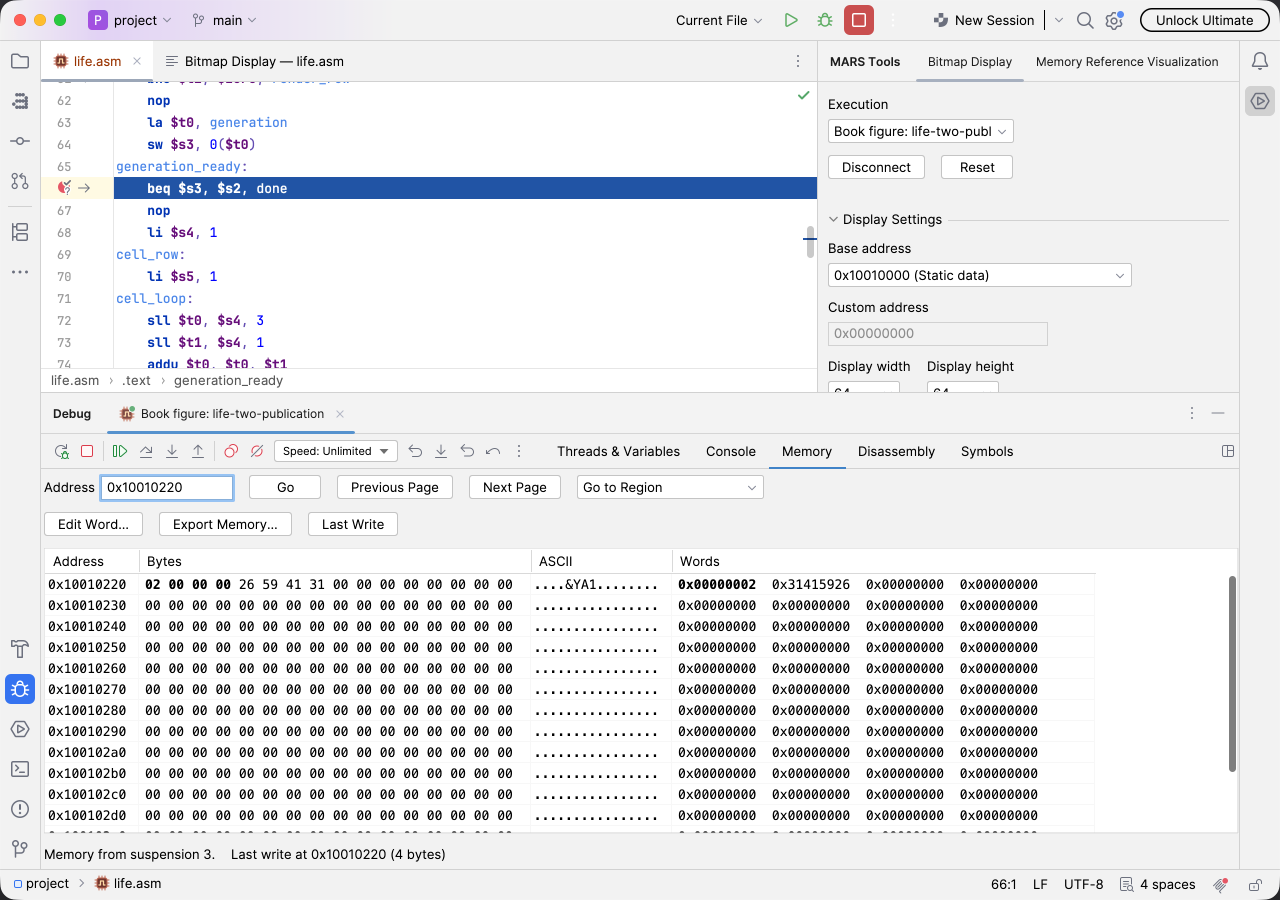
\includegraphics[artifact]{packages/008-life-generations/captures/f04-two/publication.png}}
\edef\MARStwosourceLeft{\the\dimexpr0.036718750\wd0\relax}
\edef\MARStwosourceBottom{\the\dimexpr0.774444444\ht0\relax}
\edef\MARStwosourceRight{\the\dimexpr0.611718750\wd0\relax}
\edef\MARStwosourceTop{\the\dimexpr0.147777778\ht0\relax}
\edef\MARStwostateLeft{\the\dimexpr0.246093750\wd0\relax}
\edef\MARStwostateBottom{\the\dimexpr0.075555556\ht0\relax}
\edef\MARStwostateRight{\the\dimexpr0.596875000\wd0\relax}
\edef\MARStwostateTop{\the\dimexpr0.828888889\ht0\relax}
\edef\MARStwoplotLeft{\the\dimexpr0.203906250\wd2\relax}
\edef\MARStwoplotBottom{\the\dimexpr0.066666667\ht2\relax}
\edef\MARStwoplotRight{\the\dimexpr0.203906250\wd2\relax}
\edef\MARStwoplotTop{\the\dimexpr0.091111111\ht2\relax}
\edef\MARStwomemoryLeft{\the\dimexpr0.034375000\wd4\relax}
\edef\MARStwomemoryBottom{\the\dimexpr0.334444444\ht4\relax}
\edef\MARStwomemoryRight{\the\dimexpr0.578906250\wd4\relax}
\edef\MARStwomemoryTop{\the\dimexpr0.608888889\ht4\relax}
\begin{tikzpicture}[alt={Four annotated details at generation ready with native condition s3 equals two. Current pointer s0 again selects board A and destination s1 selects board B. Both the counter and the published generation are two. The framebuffer is horizontal again, with live cells two three, three three and four three.}]
\node[anchor=north west,inner sep=0,font=\small\bfseries] (source-title) at (6mm,0) {Next instruction at the boundary};
\node[anchor=north west,inner sep=0] (source) at ([yshift=-1mm]source-title.south west) {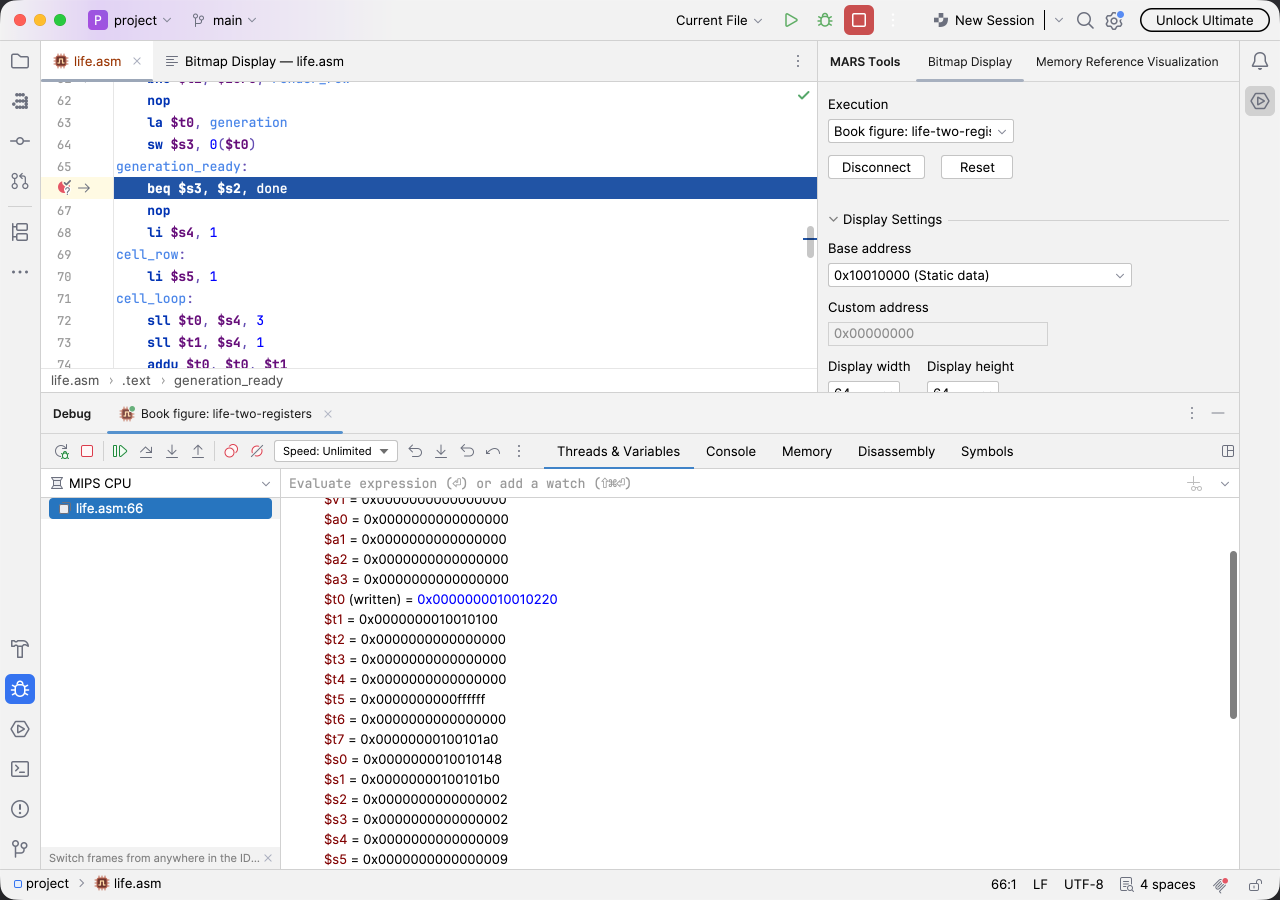
\includegraphics[width=0.7\linewidth,artifact,trim={\MARStwosourceLeft{} \MARStwosourceBottom{} \MARStwosourceRight{} \MARStwosourceTop{}},clip]{packages/008-life-generations/captures/f04-two/registers.png}};
\begin{scope}[shift={(source.south west)},x={($(source.south east)-(source.south west)$)},y={($(source.north west)-(source.south west)$)}]
\draw[black,line width=0.7pt] (0.153333333,0.057142857) rectangle (0.533333333,0.371428571);
\node[draw=black,fill=white,circle,inner sep=1.5pt,font=\footnotesize] at ($(0.153333333,0.371428571)+(-3mm,0)$) {1};
\end{scope}
\node[anchor=north west,inner sep=0,font=\small\bfseries] (state-title) at ([yshift=-2mm]source.south west) {Current and destination roles};
\node[anchor=north west,inner sep=0] (state) at ([yshift=-1mm]state-title.south west) {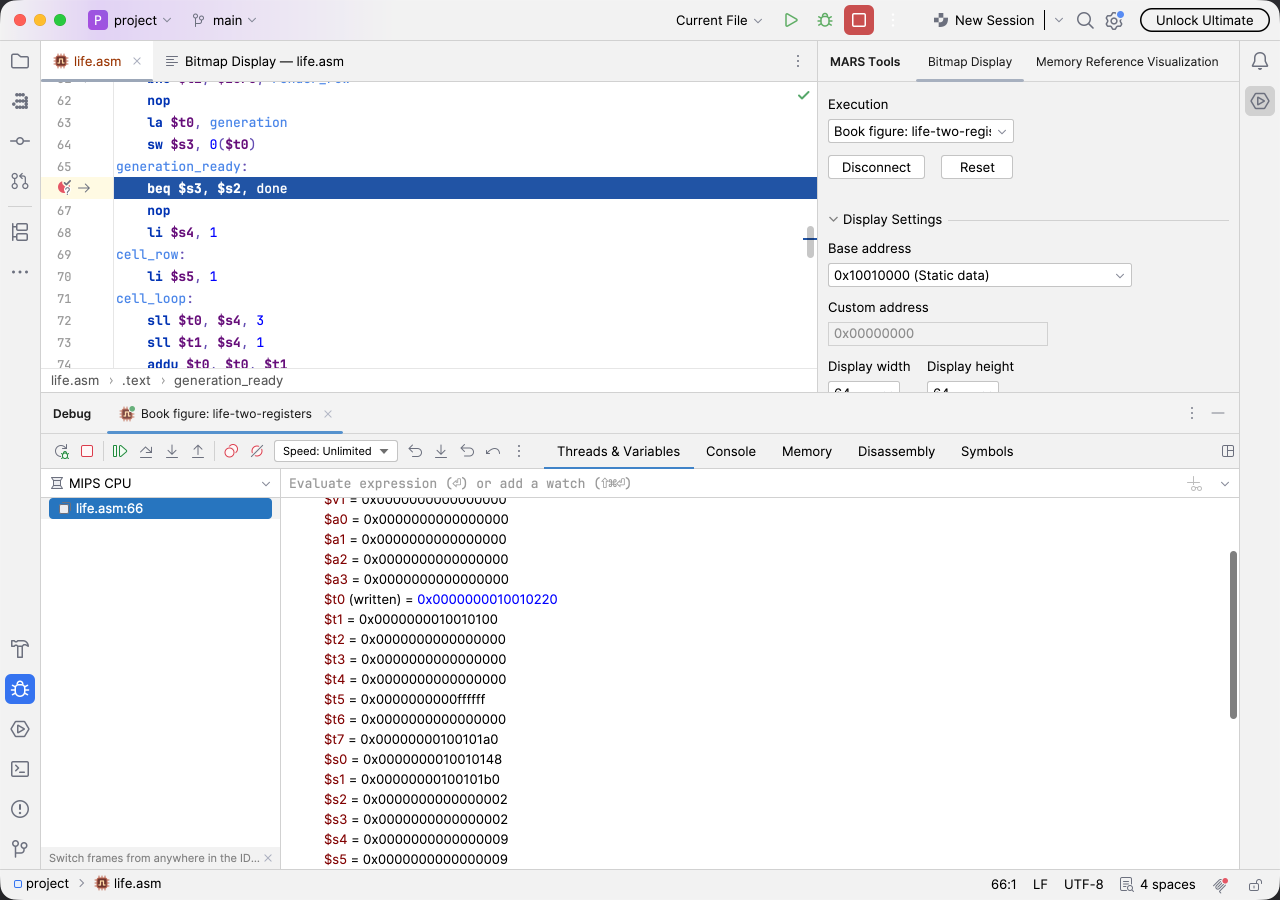
\includegraphics[width=0.4\linewidth,artifact,trim={\MARStwostateLeft{} \MARStwostateBottom{} \MARStwostateRight{} \MARStwostateTop{}},clip]{packages/008-life-generations/captures/f04-two/registers.png}};
\begin{scope}[shift={(state.south west)},x={($(state.south east)-(state.south west)$)},y={($(state.north west)-(state.south west)$)}]
\draw[black,line width=0.7pt] (0.029850746,0.034883721) rectangle (0.970149254,0.965116279);
\node[draw=black,fill=white,circle,inner sep=1.5pt,font=\footnotesize] at ($(0.029850746,0.965116279)+(-3mm,0)$) {2};
\end{scope}
\node[anchor=north west,inner sep=0,font=\small\bfseries] (plot-title) at ([xshift=0.49\linewidth]state-title.north west) {Published framebuffer};
\node[anchor=north west,inner sep=0] (plot) at ([yshift=-1mm]plot-title.south west) {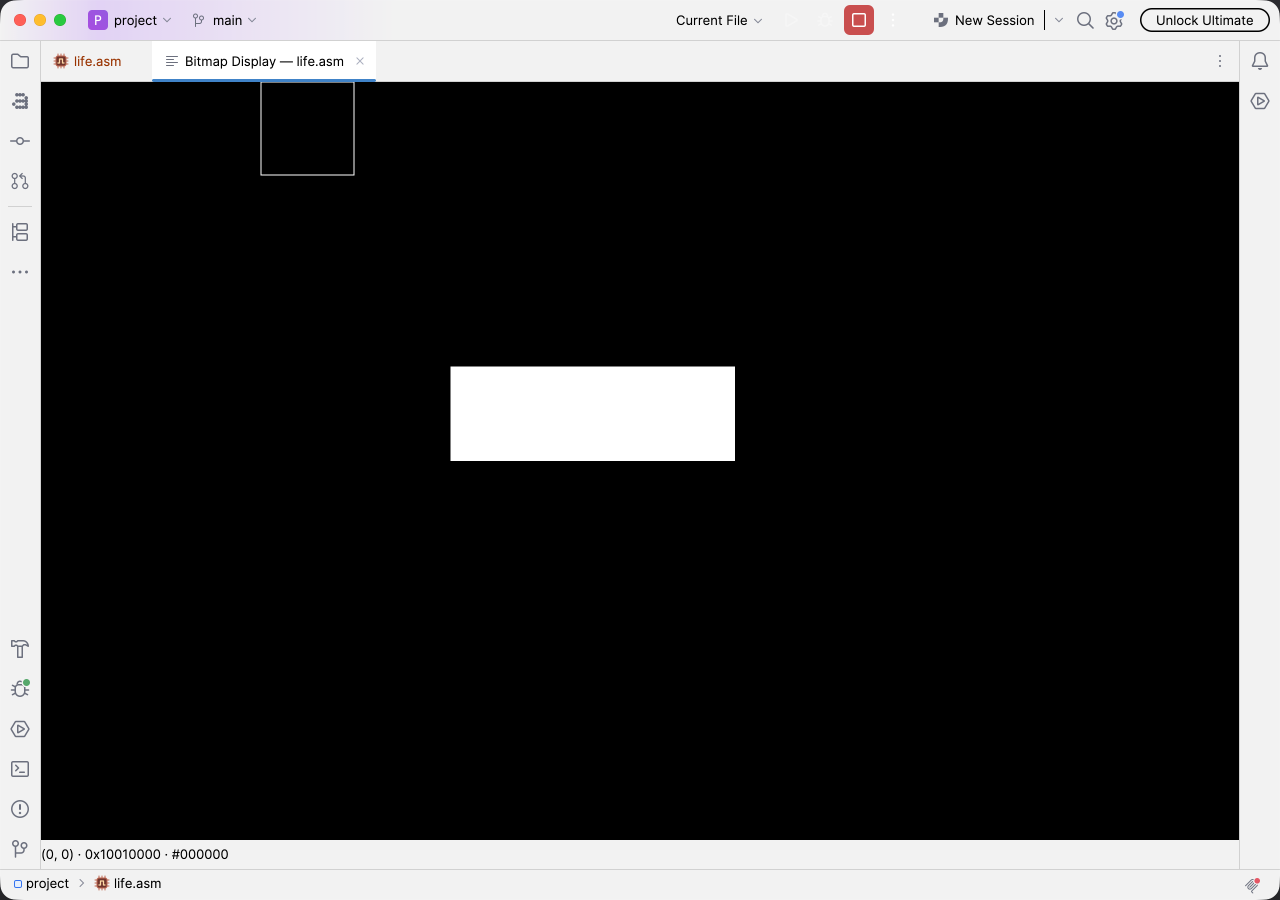
\includegraphics[width=0.32\linewidth,artifact,trim={\MARStwoplotLeft{} \MARStwoplotBottom{} \MARStwoplotRight{} \MARStwoplotTop{}},clip]{packages/008-life-generations/captures/f04-two/bitmap.png}};
\begin{scope}[shift={(plot.south west)},x={($(plot.south east)-(plot.south west)$)},y={($(plot.north west)-(plot.south west)$)}]
\draw[black,line width=0.7pt] (0.000000000,0.000000000) rectangle (1.000000000,1.000000000);
\node[draw=black,fill=white,circle,inner sep=1.5pt,font=\footnotesize] at ($(0.000000000,1.000000000)+(-3mm,0)$) {3};
\foreach \c in {0,...,7} {\node[anchor=north,font=\scriptsize,inner sep=0] at ({(\c+0.5)/8},-0.035) {\c}; \node[anchor=east,font=\scriptsize,inner sep=0] at (-0.025,{1-(\c+0.5)/8}) {\c};}
\node[anchor=north,font=\scriptsize,inner sep=0] at (0.5,-0.11) {$x$}; \node[anchor=east,font=\scriptsize,inner sep=0] at (-0.10,0.5) {$y$};
\end{scope}
\node[anchor=north west,inner sep=0,font=\small\bfseries] (memory-title) at ([yshift=-9mm]state-title.north west |- plot.south west) {Published generation, then its guard};
\node[anchor=north west,inner sep=0] (memory) at ([yshift=-1mm]memory-title.south west) {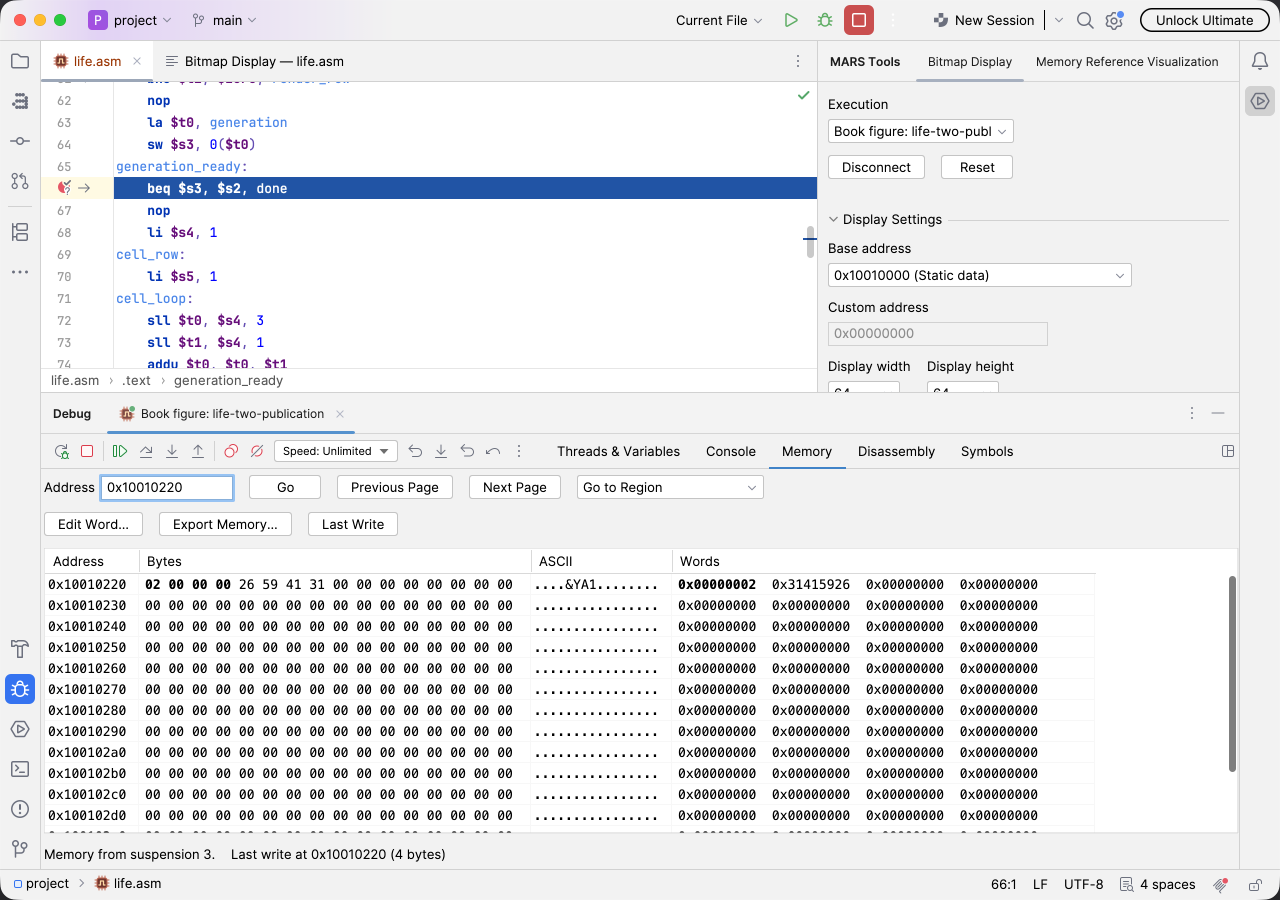
\includegraphics[width=0.78\linewidth,artifact,trim={\MARStwomemoryLeft{} \MARStwomemoryBottom{} \MARStwomemoryRight{} \MARStwomemoryTop{}},clip]{packages/008-life-generations/captures/f04-two/publication.png}};
\begin{scope}[shift={(memory.south west)},x={($(memory.south east)-(memory.south west)$)},y={($(memory.north west)-(memory.south west)$)}]
\draw[black,line width=0.7pt] (0.191919192,0.078431373) rectangle (0.983838384,0.490196078);
\node[draw=black,fill=white,circle,inner sep=1.5pt,font=\footnotesize] at ($(0.191919192,0.490196078)+(-3mm,0)$) {4};
\end{scope}
\end{tikzpicture}
\par\smallskip
\begin{minipage}{\linewidth}
\small
\begin{enumerate}
\item The condition \texttt{\$s3 == 2} selects the third visit. The next \texttt{beq} compares equal counters and will branch to \texttt{done}; it does not begin a third update.
\item Two swaps return the current pointer to A at \texttt{0x10010148}. B at \texttt{0x100101b0} retains generation one and becomes the unused destination. Equal pointer roles at generations zero and two do not mean that no computation occurred.
\item The horizontal pattern matches generation zero exactly. This blinker has period two. The image alone cannot identify which generation is published; the source boundary, working counter and publication bytes supply that information.
\item The bytes \texttt{02 00 00 00} publish generation two, and the adjacent guard is unchanged. Both requested updates and all three renders are complete. The final frame remains visible when normal exit follows.
\end{enumerate}
\end{minipage}
\caption{Generation two returns to board A and repeats the seed pattern.}
\label{capture:008-life-generations-f04-two}
\end{figure}
\par
